\documentclass{beamer}
\usetheme{CambridgeUS}
\usecolortheme{dolphin} 
\usepackage[utf8]{inputenc}
\usepackage[spanish]{babel}
\usepackage{graphicx}
\usepackage{listings}

\title[Tecnologia]
{Tercer Intento}
\subtitle{Falta de exclusion mutua}
\author[Grupo 1] 
{Ignacio P\'erez Laborda\\B\'arbara Mart\'inez}
\institute[UB--FTI] 
{
  Facultad de Tecnolog\'ia Inform\'atica\\
  Universidad de Belgrano
}
\date[\today] 

\renewcommand{\thefootnote}{\roman{footnote}}

\begin{document}
%1
%\frame{\titlepage}

\begin{frame}


\includegraphics[height=0.2\textheight]{ub2.jpg} \hspace*{6cm}

\includegraphics[height=0.19\textheight]{FTI.jpg}  
\\[-0.1cm]
\titlepage


\end{frame}

\begin{frame}{Introducción}

\begin{enumerate}[$*$]
\item El problema principal de la alternancia se produce porque no se puede conservar la suficiente cantidad de informacion acerca del estado de cada proceso.
\item   Solo es posible recordar cual es el proceso al cual se le permite entrar a la seccion crítica
\item  Se solucionó este problema colocando 2 variables compartidas asociadas cada una a su proceso 
\end{enumerate}

\end{frame}

\begin{frame}[fragile]

\frametitle{Imagen explicativa sobre la exclusion mutua} \vspace*{-0.8 cm}
 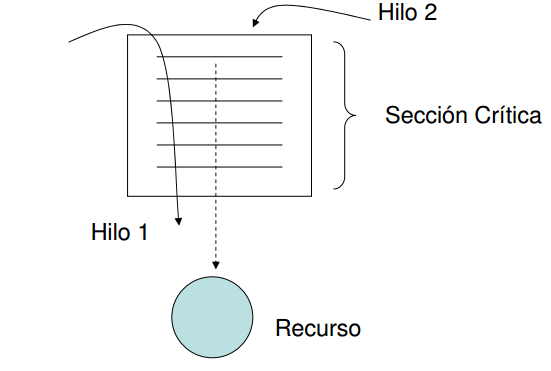
\includegraphics[width=0.8\textwidth]{exclmu.png}

\end{frame}


\begin{frame}[fragile]

\frametitle{Código fuente del Algoritmo: Clase almacén}\vspace*{-0.3cm}
\lstset{language=,emph={if, else},emphstyle=\textbf}

\begin{lstlisting}
class almacen { 
    int[] almacen = new int[16]; 
    int primero = 0; 
    int cuantos = 0;

    synchronized public int coger() { 
       int aux; 
       if (cuantos == 0) 
           return (-1); 
       else { 
           cuantos--; 
           aux = primero; 
           primero = (primero + 1) & 15; 
           return(almacen[aux]); 
       } 
    }
  
\end{lstlisting}
\end{frame}

\begin{frame}[fragile]

\frametitle{Código fuente del Algoritmo: Clase almacén(Continuación)}\vspace*{-0.5cm}
\lstset{language=,emph={if, else},emphstyle=\textbf}

\begin{lstlisting}
class almacen { 
   synchronized public boolean dejar(char val) { 
       if (cuantos == 16) 
           return false; 
       int aux; 
       aux = (primero + cuantos) & 15; 
       cuantos++; 
       almacen[aux] = val; 
       return true; 
    } 
} // almacen


\end{lstlisting}
\end{frame}


\begin{frame}

\frametitle{Descripcion del algoritmo}
Al ejecutarse el proceso y después de realizar sus tareas iniciales, verifica si otro proceso esta dentro de la sección critica 
\par Si el otro proceso esta dentro entonces espera a que salga de la sección critica. De lo contrario pasa la fase de comprobación y cambia su estado a que esta dentro 
\par Luego de pasar la sección critica cambia su estado, termina sus tareas finales.


\end{frame}

\begin{frame}

\frametitle{Problemas del algoritmo}
\begin{enumerate}[$*$]
\item Se corre el riesgo de producir un interbloqueo si dos procesos tienen un flag true: al querer acceder las dos variables al mismo recurso ninguna puede hacerlo.
\item    A su ves se produce una no progresión , ya que no hay forma de revertir lo ocurrido
\item  Todavia sigue sin resolverse el problema de que si un proceso se interrumpe mientras queda ejecutada su sección crítica , el otro queda bloqueado tmb
\end{enumerate}

\end{frame}



\end{document}

